\subsection{Thermal Expansion Analysis}

The fuel and cladding form a coupled system, with the gap between them playing a critical role in heat transfer, mechanical interactions, and overall reactor safety. Accurate evaluation of thermal expansion is essential to ensure efficient operation and structural integrity of the reactor core. These calculations account for material-specific thermal expansion coefficients and the temperature distributions derived from operational data.

\subsubsection{Axial Temperature Profile of the Fuel and Axial Profile of Fuel Radius (Cold vs. Hot Geometry)}

The axial temperature profile of the fuel under hot operational conditions is shown in Figure~\ref{fig:Fuel_Temperature_Hot}. This profile provides insight into the temperature distribution along the fuel height, which is essential for evaluating thermal stresses and expansion. The corresponding axial profile of the fuel radius, depicted in Figure~\ref{fig:Fuel_Radius_ColdHot}, demonstrates that the material’s expansion aligns closely with the temperature distribution.

\begin{figure}[H]
\centering
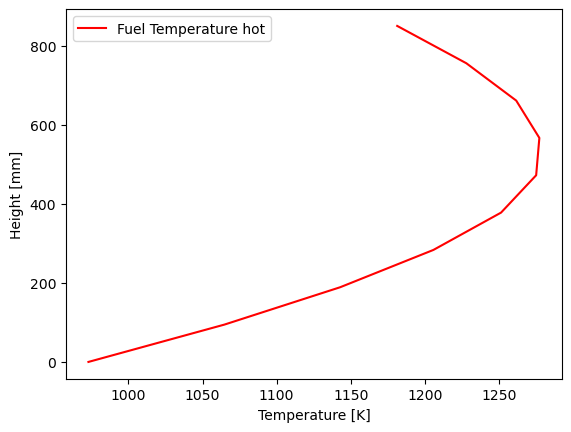
\includegraphics[width=0.8\textwidth]{1a_fuel_hot.png}
\caption{Axial temperature profile of the fuel under hot operational conditions.}
\label{fig:Fuel_Temperature_Hot}
\end{figure}

\begin{figure}[H]
\centering
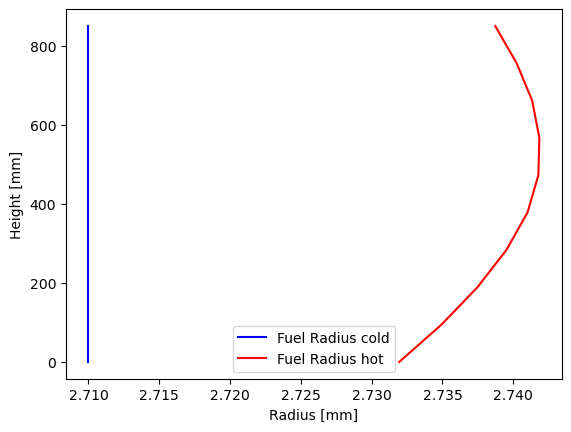
\includegraphics[width=0.8\textwidth]{1b_fuel_coldhot.png}
\caption{Axial profile of the fuel radius (cold vs. hot geometry).}
\label{fig:Fuel_Radius_ColdHot}
\end{figure}

\subsubsection{Axial Temperature Profile of the Inner and Outer Cladding (Cold vs. Hot Geometry)}

The axial temperature profiles of the cladding’s inner and outer surfaces illustrate the thermal distribution along its height. Figure~\ref{fig:Cladding_InOut_Temperature_Hot} highlights the uniform expansion of the cladding along its axial height. The temperature difference between the inner and outer surfaces remains consistent, as shown in Figure~\ref{fig:Cladding_Radius_ColdHot}.

\begin{figure}[H]
\centering
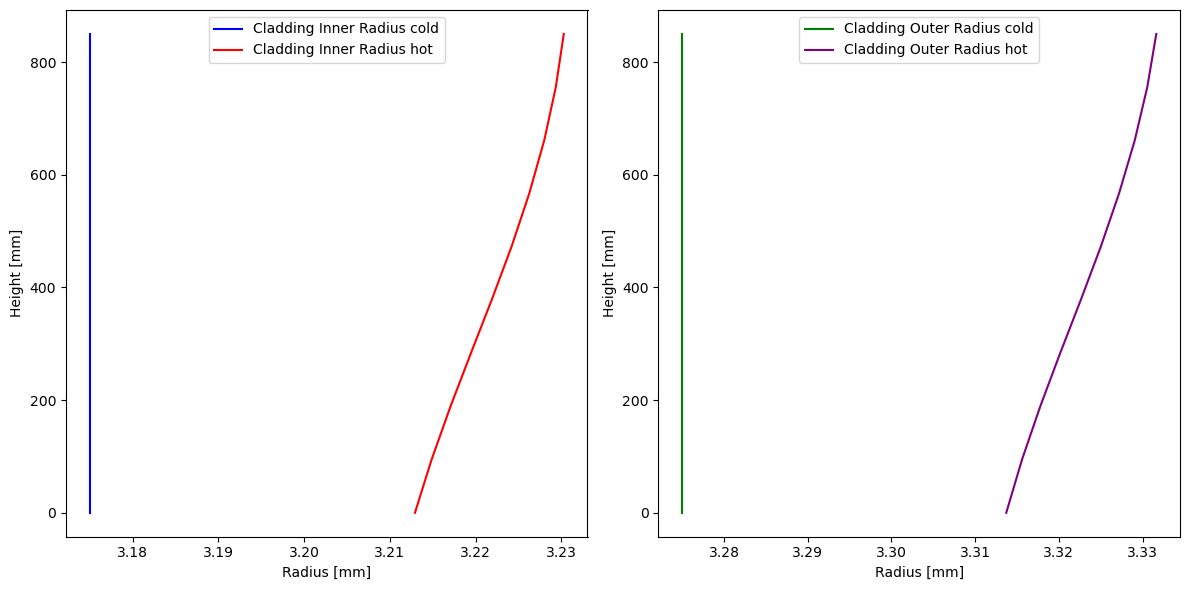
\includegraphics[width=0.8\textwidth]{2_cladding_in_out_coldhot.png}
\caption{Axial temperature profile of the cladding (cold vs. hot geometry).}
\label{fig:Cladding_InOut_Temperature_Hot}
\end{figure}

\begin{figure}[H]
\centering
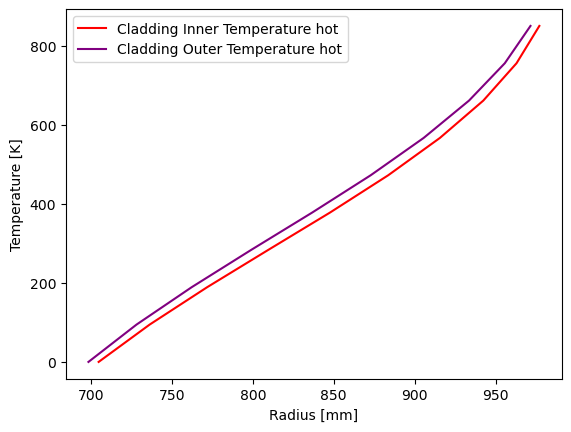
\includegraphics[width=0.8\textwidth]{3_clad_inout_diff.png}
\caption{Axial profile of the cladding radius (cold vs. hot geometry).}
\label{fig:Cladding_Radius_ColdHot}
\end{figure}

\subsubsection{Gap and Cladding Thickness Along Axial Height}

The evolution of the fuel-cladding gap due to differential expansion is presented in Figure~\ref{fig:Gap_Cladding_Thickness}. This parameter significantly influences heat transfer efficiency and mechanical interactions in the reactor core. While the change in cladding thickness with temperature is relatively minor compared to the change in radius, it remains a critical factor for evaluating structural integrity.

\begin{figure}[H]
\centering
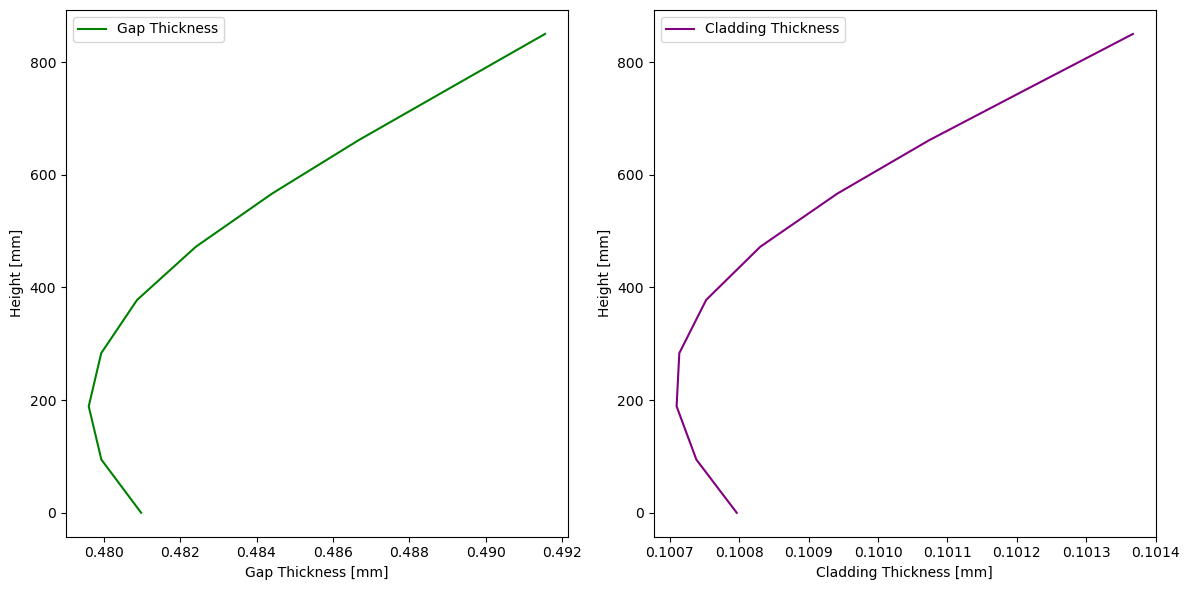
\includegraphics[width=0.8\textwidth]{4_gap_clad_thickness.png}
\caption{Gap and cladding thickness along the axial height.}
\label{fig:Gap_Cladding_Thickness}
\end{figure}

\subsubsection{Discussion}

As anticipated, the fuel exhibits more pronounced thermal expansion due to its higher temperature gradient compared to the cladding. This results in a reduction of the gap between the fuel and cladding, enhancing thermal coupling. However, careful management of this reduced gap is necessary to prevent mechanical interactions that could compromise the system's structural integrity.
